\section{Systematic Errors}

% ------------ section structure -------------
% (a) summary of the systematic errors and their relative size 
% (b) description of different sources of error (fits, data inconsistany, cut choices)
% -------------------------------------------

The error on our measured values is considered in two categories.  First, statistical errors are calculated for the beam spin asymmetry measurement for every phi-bin.  During the fitting procedure, these statistical errors are mapped into errors on the fit parameters.  This first class of errors we consider as the statistcal error on the result.  Second, the authors consider all other possible sources of error which do not depend on statistical effects.  Those effects which have been identified are: \\


\begin{center}
\begin{tabular}{ | c || c |  }
 \hline
 Source & Relative Error\\
 \hline
 Cut: z-vertex                   & 0.0019\\
 Cut: \texttt{EC edep}           & 0.0027\\
 Cut: sampling fraction          & 0.0010\\
 Cut: $\theta_{CC}$ matching     & 0.0022\\
 Cut: pion significance $\alpha$ & 0.0049\\
 Beam Polarization               & 0.03  \\
 \hline
\end{tabular}
\end{center}

\subsection{Cut Variations}
In some cases, the direct variation of analyses parameters is the only way to try and understand the dependence of the result on the input parameters.  Ideally, the analysis result shouldn't vary outside of the errors which arise from statical fluctuations.    

\begin{figure}
  \begin{center}
    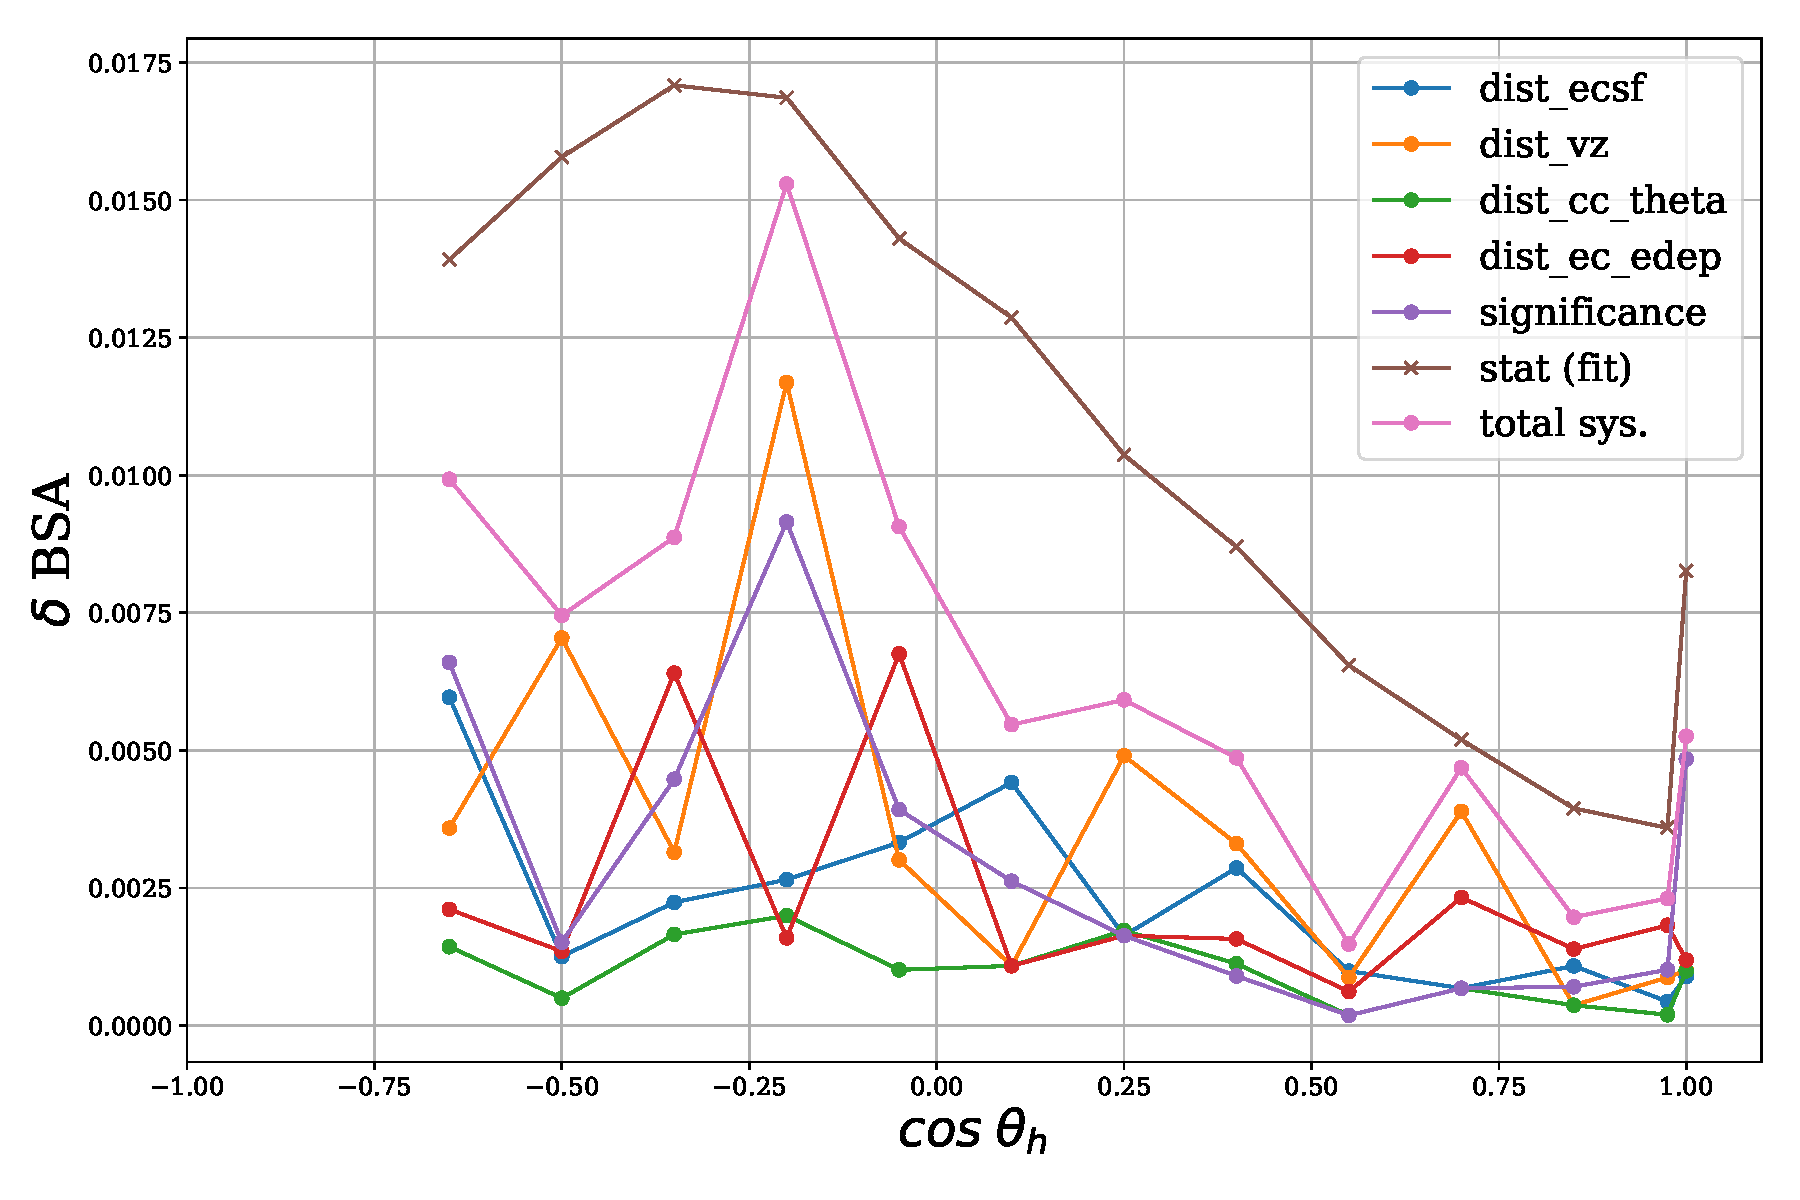
\includegraphics[width=12cm]{image/systematics.pdf}
    \caption{The largest shift resulting from all variations of each analysis cut parameter.  Shown also is the statistical error.  All resulting cut variations remained withtin statistical error.}
  \end{center}
\end{figure}

\subsection{Random Subset/Helicity}

Two additional studies are performed which involve randomization of the input data in some way.  In the first study, the helicity of each event is assigned a random value of $\pm 1$.  This randomization destroys the correlation between beam spin and the $\phi_h$ distributions.  Therefore, one expects to find zero asymmetries as a result of this randomization.  In the second study, the full analysis is run on a subset of 80\% of the events in the full dataset.  This study is designed to identify if there is internal inconsistancy in the dataset.
\\

\begin{figure}
  \begin{center}
    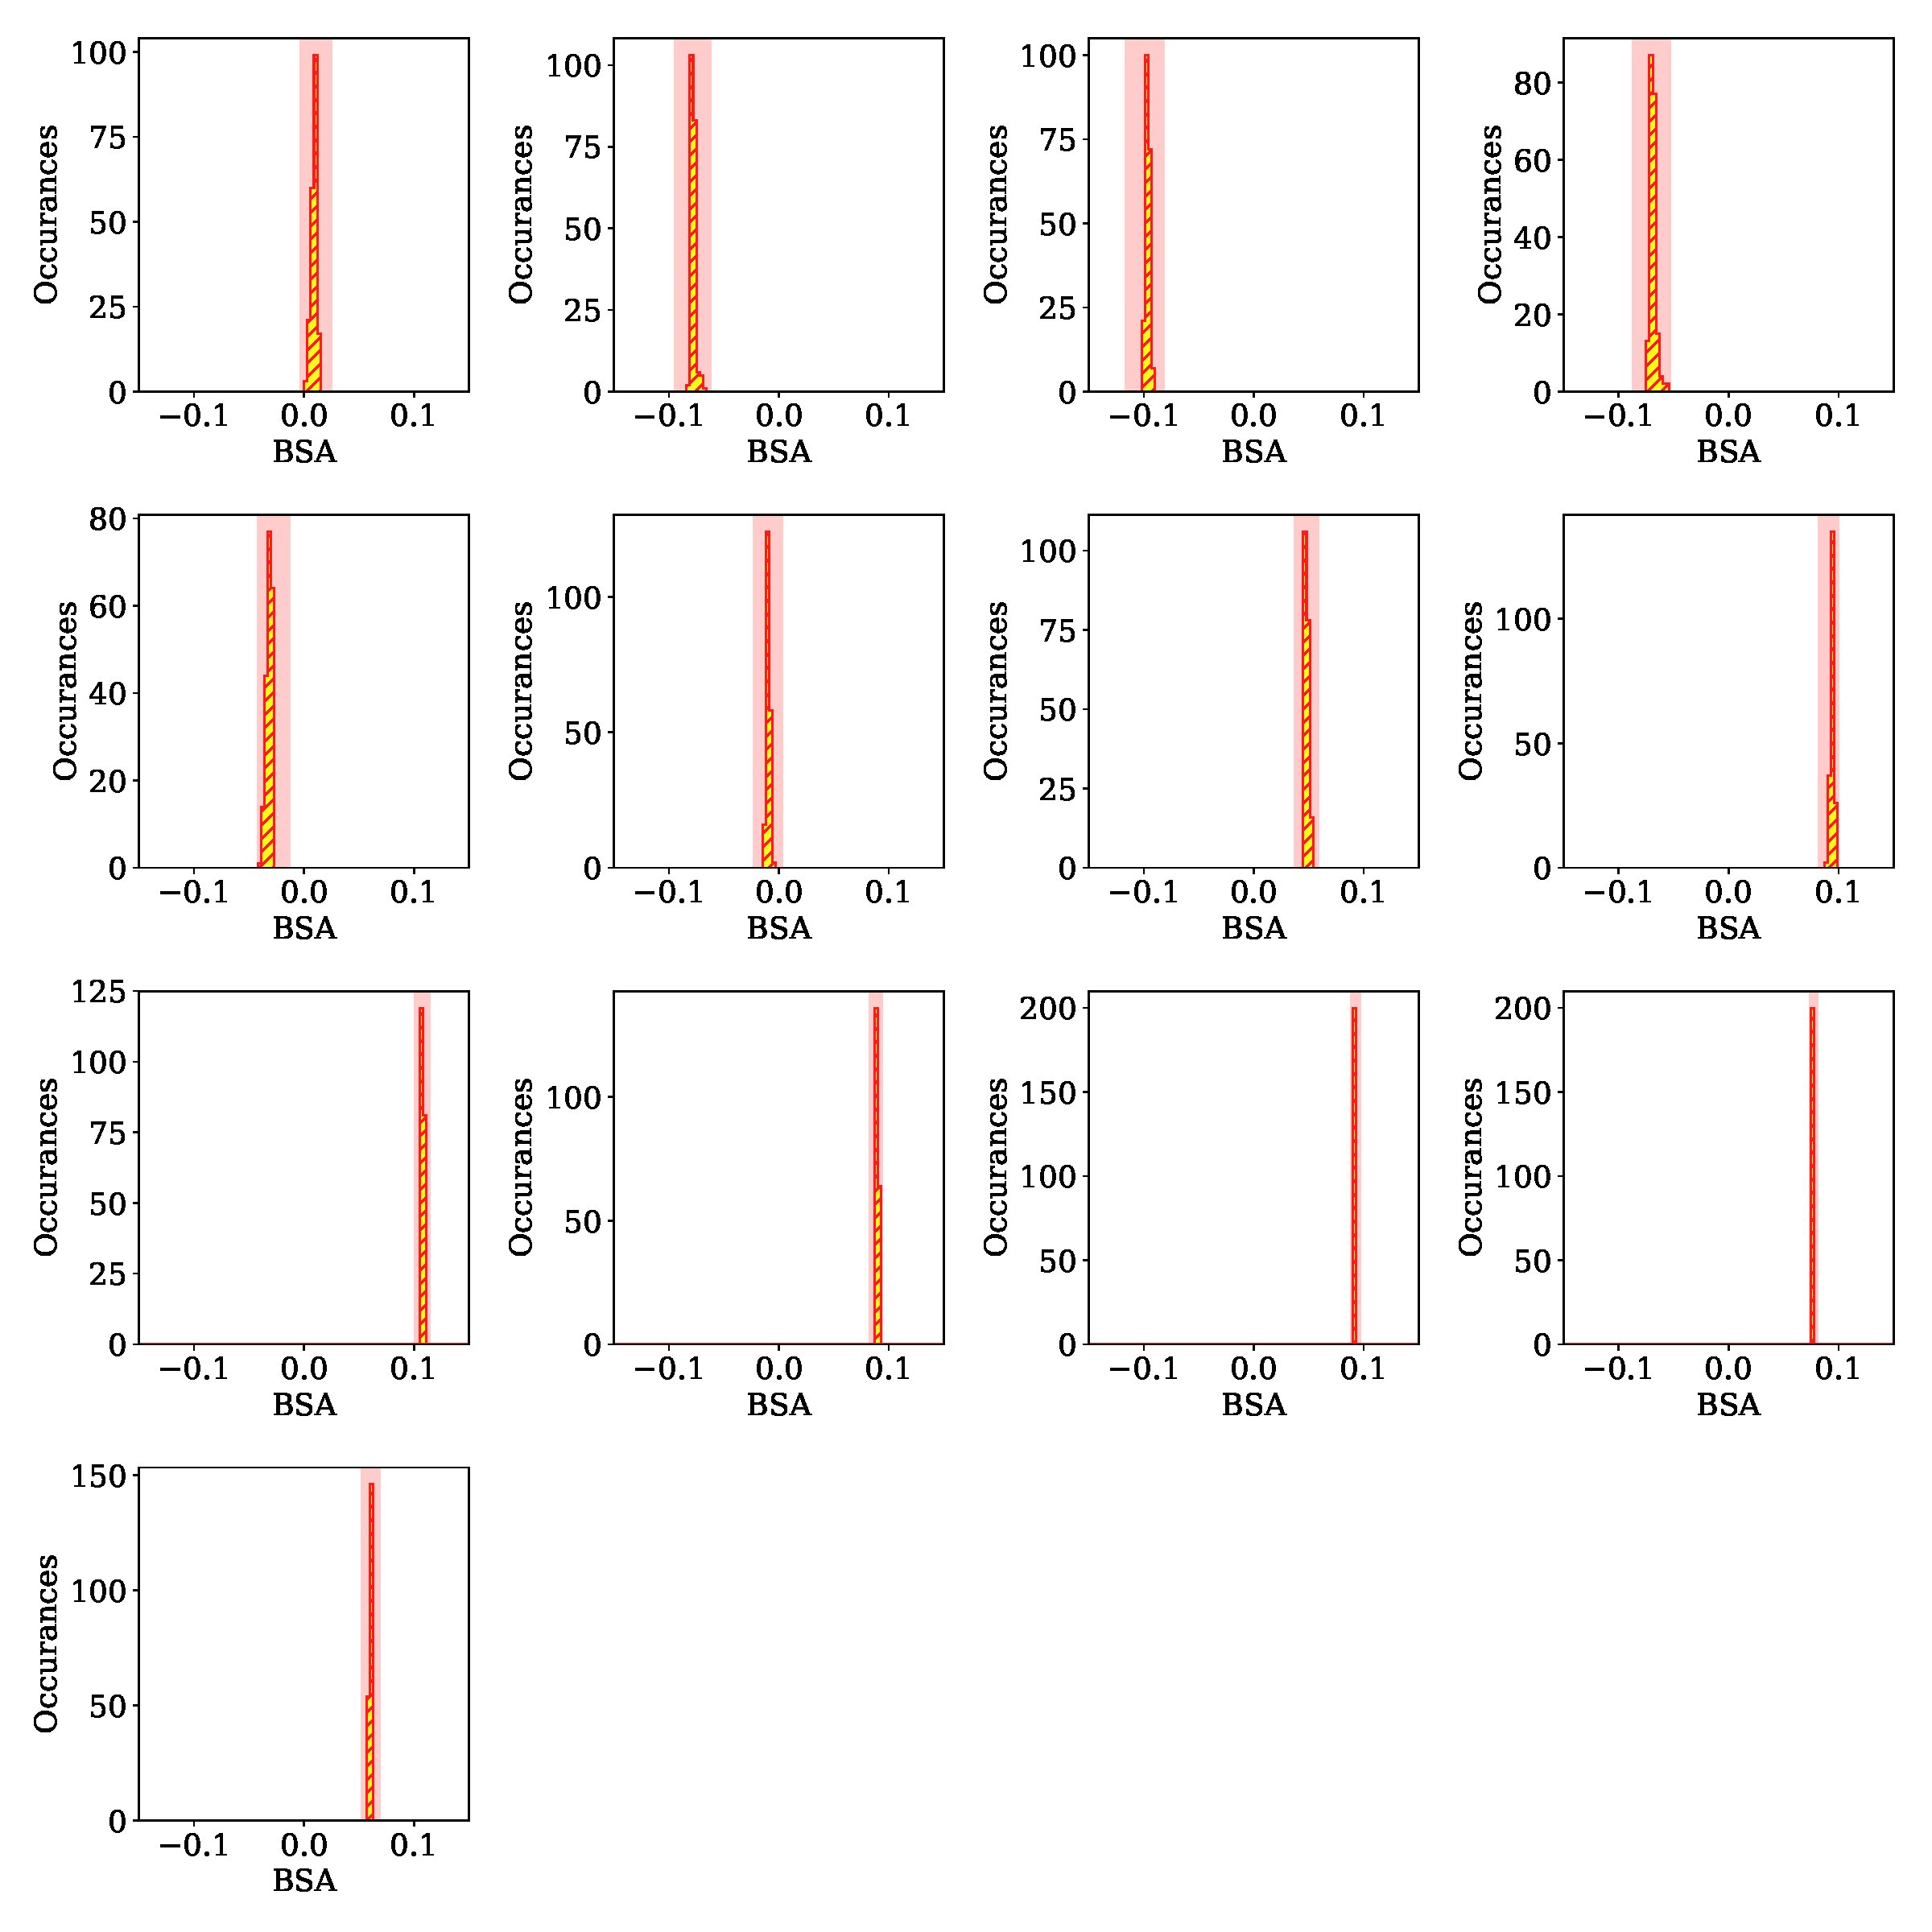
\includegraphics[width=\columnwidth]{image/subsets.pdf}
    \caption{PPPP}
  \end{center}
\end{figure}

\begin{figure}
  \begin{center}
    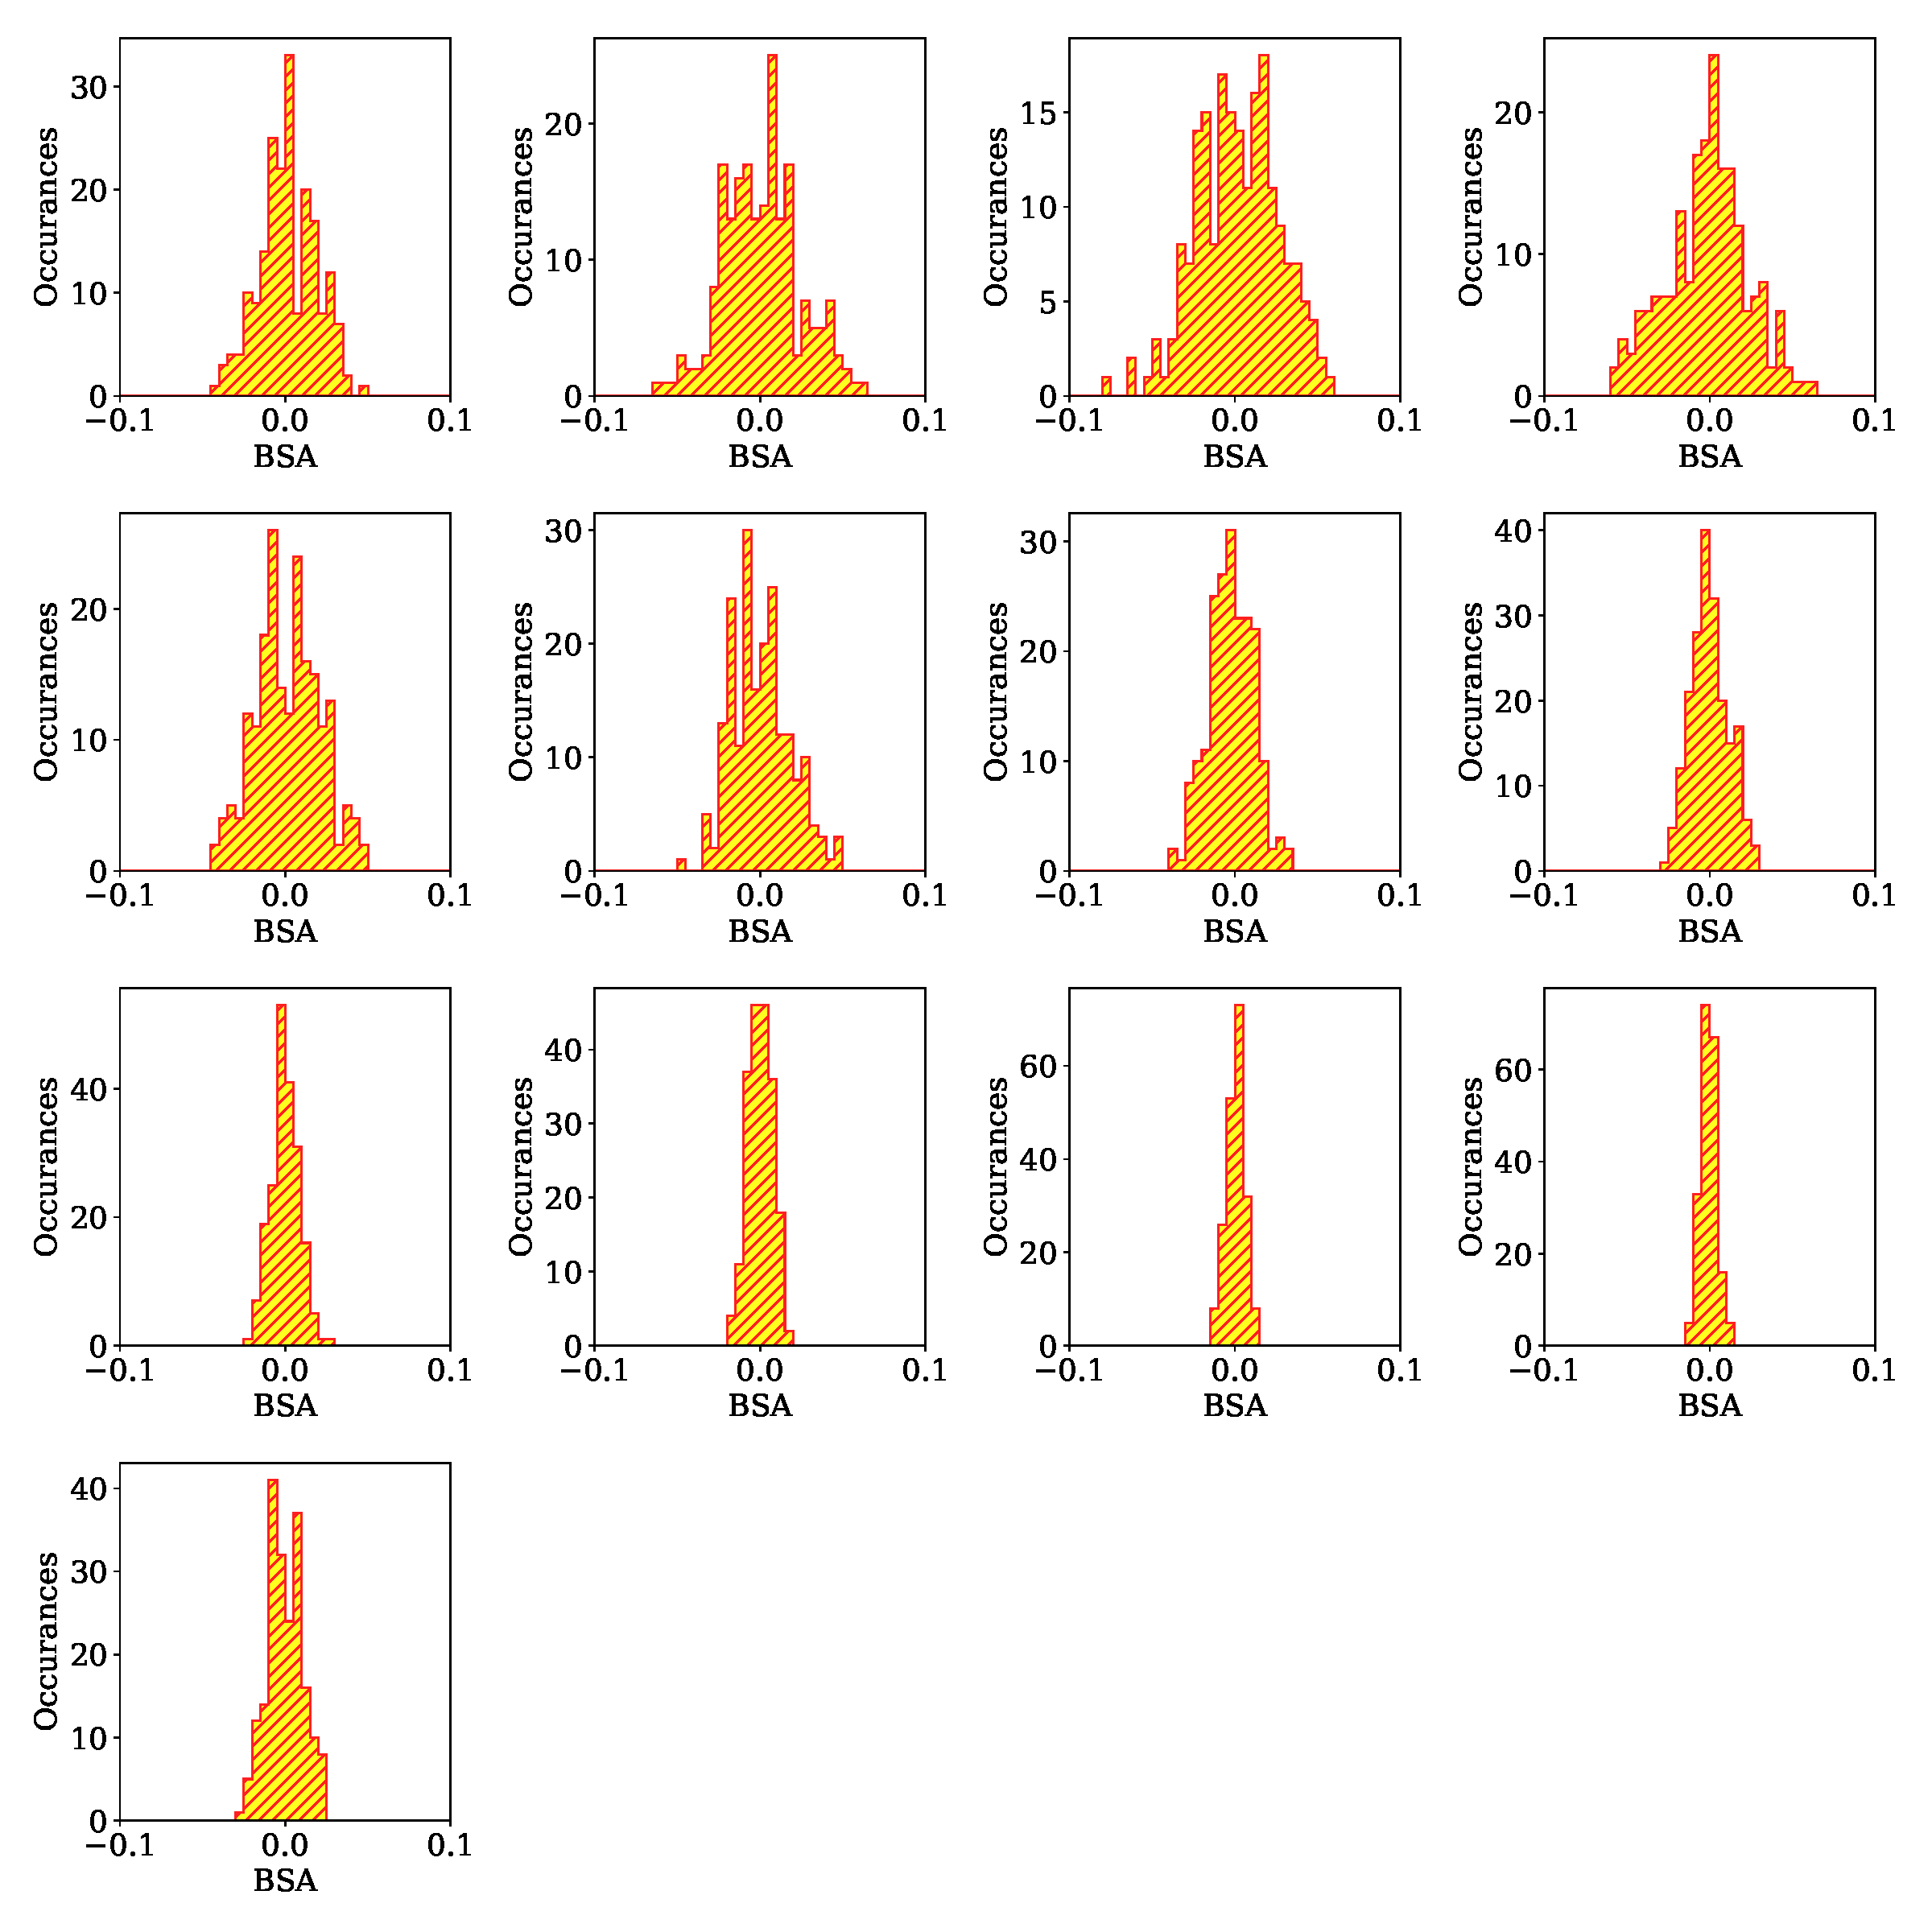
\includegraphics[width=\columnwidth]{image/helicity.pdf}
    \caption{XGDFG}
  \end{center}
\end{figure}

